\begin{figure}[H]\caption[Distribuciones]{Existe diversidad de distribuciones para modelar v.a.s, a continuación se muestran las mas importantes de acuerdo a \citeauthor{bala20} (\citeyear{bala20}).}\label{FIG:DISTS}
\begin{subfigure}[t]{.475\textwidth}\includegraphics[width=1\linewidth]{binominal.png}
Binominal $b(n,p)$. Número de éxitos en $n$ ensayos de Bernoulli independientes con la misma probabilidad de éxito $p$.
\begin{equation}\begin{matrix}
f(x=k)=\binom{n}{x}p^xp^{n-x},\\
x=0,1,\ldots,n;\\
E(X)=np,\ Var(X)=npq
\end{matrix}\end{equation}\end{subfigure}\qquad
\begin{subfigure}[t]{.475\textwidth}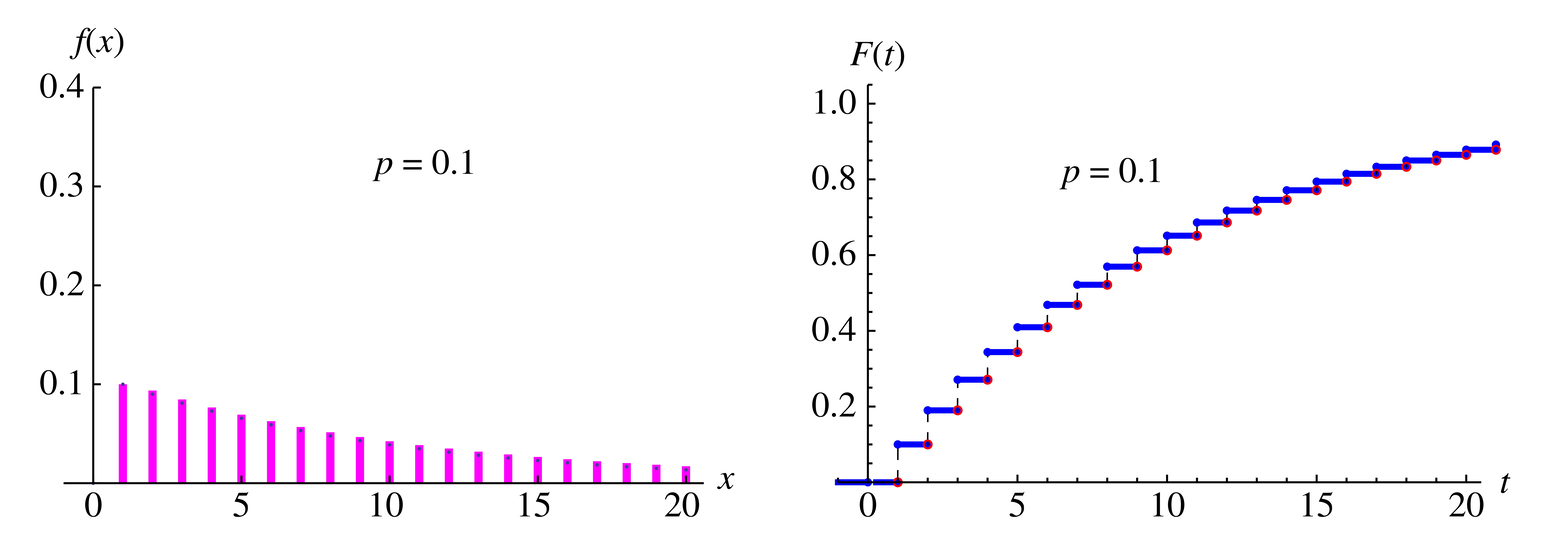
\includegraphics[width=1\linewidth]{geom.png}
Geométrica $G(p)$.
Número $n$ de ensayos de Bernoulli independientes con la misma probabilidad de éxito $p$, hasta obtener el primer éxito.
\begin{equation}\begin{matrix}
f(x)=q^{x-1},\\
x=1,2,\ldots,n;\\
E(X)=\frac{1}{p},\ Var(X)=\frac{q}{p^2}
\end{matrix}\end{equation}\end{subfigure}
\end{figure}


\begin{figure}[H]
\begin{subfigure}[t]{.475\textwidth}\includegraphics[width=1\linewidth]{negativabinominal.png}
Negativa binominal $Nb(rp)$. Número $n$ de ensayos de Bernoulli independientes con la misma probabilidad de éxito $p$, hasta obtener resultado número $r$.
\begin{equation}\begin{matrix}
f(x)=\binom{x-1}{r-1}p^rq^{x-r},\\
r=r,r+1,r+2,\ldots,n;\\
E(X)=\frac{r}{p},\ Var(X)=\frac{rq}{p^2}
\end{matrix}\end{equation}\end{subfigure}\qquad
\begin{subfigure}[t]{.475\textwidth}\includegraphics[width=1\linewidth]{hyperg.png}
Hipergeométrica $h(n;a,b)$. Muestra aleatoria tamaño $n$ de elementos tipo $a$ no reemplazada de un universo con elementos tipo $a$ y $b$.
\begin{equation}\begin{matrix}
f(x)=P(X=x)=\frac{\binom{a}{x}\binom{b}{n-x}}{\binom{a+b}{n}};\\
E(X)=n\cdot\frac{a}{a+b},\\
Var(X)=n\cdot\frac{a}{a+b}\cdot\frac{b}{a+b}\cdot(1-\frac{n-1}{a+b-1})
\end{matrix}\end{equation}\end{subfigure}
\end{figure}


\begin{figure}[H]
\begin{subfigure}[t]{.475\textwidth}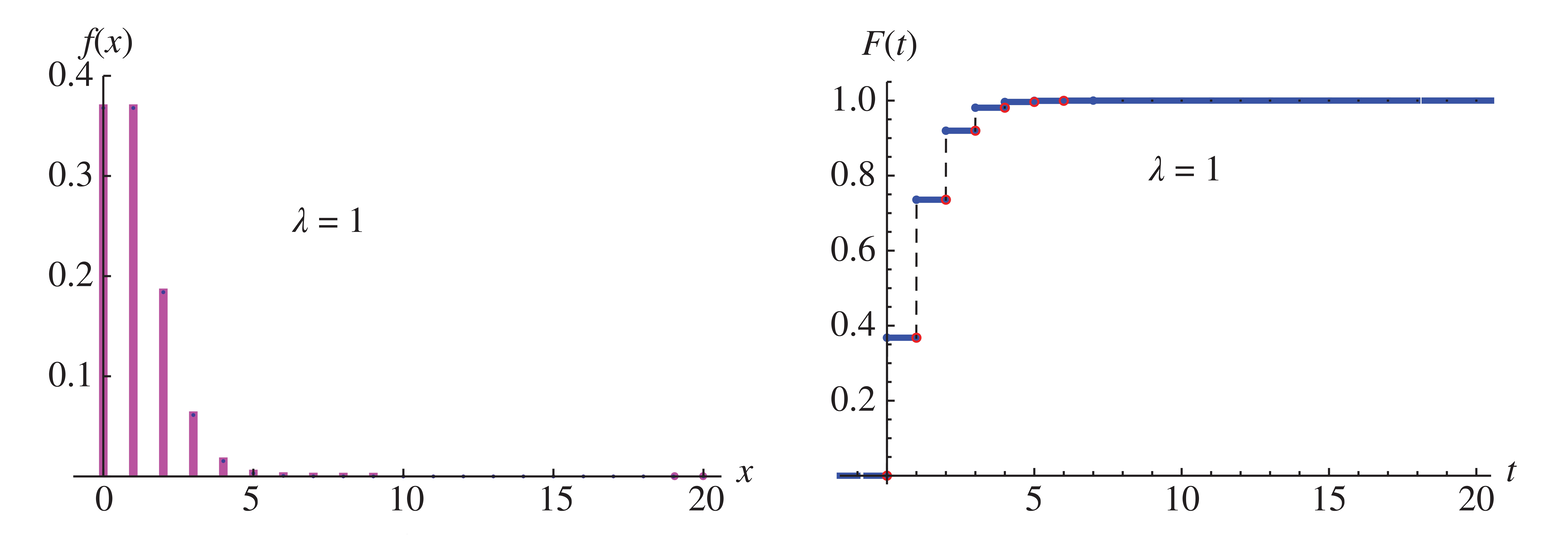
\includegraphics[width=1\linewidth]{poisson.png}
Poisson $\mathcal{P}(\lambda)$. Puede utilizarse con algún parámetro $\lambda$ cuando la probabilidad de éxito tiende a cero $(p\rightarrow0)$ de forma que la media $E(X)=np$ converge en algún $\lambda>0$.
\begin{equation}\begin{matrix}
f(x)=e^{-\lambda}\frac{\lambda^x}{x!},\\
x=0,1,2,\ldots;\\
E(X)=\lambda, Var(X)=\lambda
\end{matrix}\end{equation}\end{subfigure}\qquad
\begin{subfigure}[t]{.475\textwidth}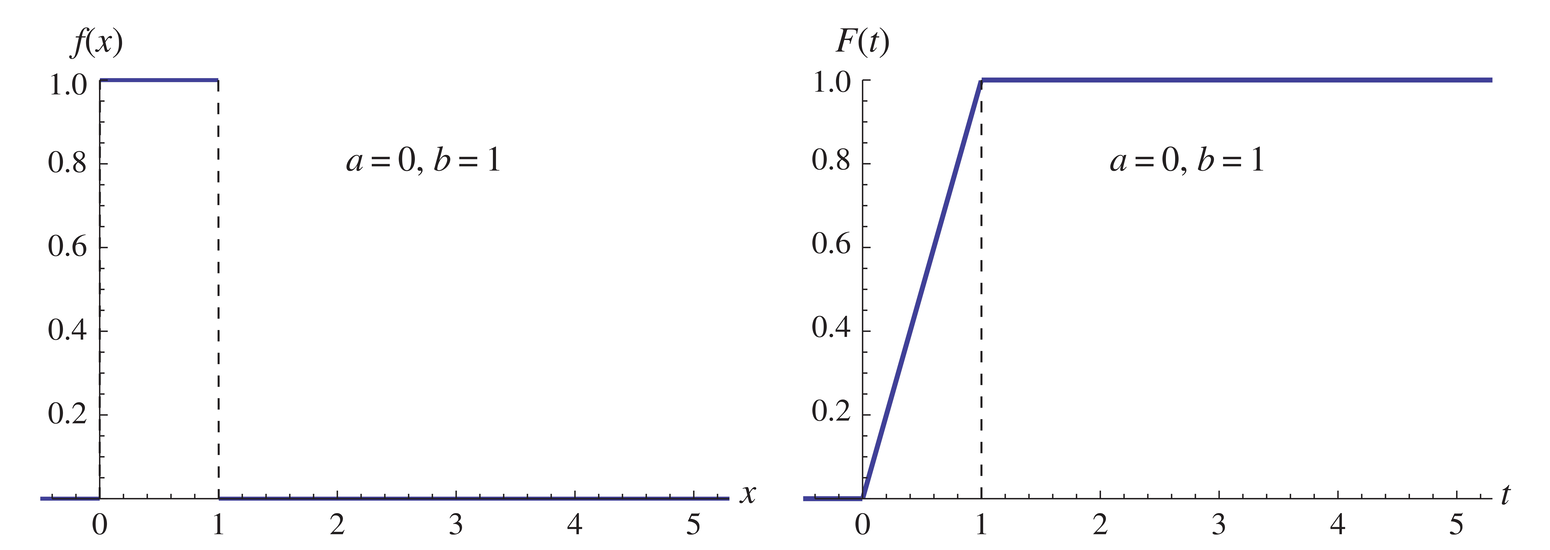
\includegraphics[width=1\linewidth]{uniforme.png}
Uniforme $U[a,b]$. Útil para modelar situaciones en que todos los intervalos tengan la misma amplitud y probabilidad.
\begin{equation}\begin{matrix}
f(x)\begin{cases}\frac{1}{b-a},\quad a\leq x\leq b,\\\text{de otro modo},\quad 0;\end{cases}\\
F(t)\begin{cases}0,\quad t<0,\\\frac{t-a}{b-a},\quad a\leq t\leq b,\\1,\quad t>b;\end{cases}\\
E(X)=\frac{a+b}{2},\quad Var(X)=\frac{{(b-a)}^2}{12}
\end{matrix}\end{equation}\end{subfigure}
\end{figure}


\begin{figure}[H]
\begin{subfigure}[t]{.475\textwidth}\includegraphics[width=1\linewidth]{normal.png}
Normal $N(\mu,\sigma^2)$. La suma y el promedio de un gran número de observaciones para una variable $X$ puede ser aproximada por la distribución normal, independientemente de su distribución original.
\begin{equation}\begin{matrix}
f(x)=\frac{1}{\sigma\sqrt{2\pi}}e^{-({x-\mu)}^2/(2\sigma^2)},\\
-\infty<z<\infty;\\
E(X)=\mu,\ Var(X)=\sigma^2
\end{matrix}\end{equation}\end{subfigure}\qquad
\begin{subfigure}[t]{.475\textwidth}\includegraphics[width=1\linewidth]{epsilon_lambda.png}
Exponencial $\epsilon(\lambda)$. Es considerada la análoga continua de la distribución geométrica y puede ser utilizada para modelar parte de la vida de un sujeto $X$.
\begin{equation}\begin{matrix}
f(x)=\begin{cases}\lambda^{-\lambda x},\ x\leq0,\\0,\ x<0;\end{cases}\\
F(t)=\begin{cases}0,\ t<0,\\1-e^{-\lambda t},\ x\geq 0;\end{cases}\\
E(X)=\frac{1}{\lambda},\ Var(X)=\frac{1}{\lambda^2}
\end{matrix}\end{equation}\end{subfigure}
\end{figure}

\begin{figure}[H]
\begin{subfigure}[t]{.475\textwidth}\includegraphics[width=1\linewidth]{gama.png}
Gama. Generalización de la distribución \emph{Erlang} cuando el parámetro $n$ no es necesariamente un entero.
\begin{equation}\begin{matrix}
f(x)=\begin{cases}\frac{\lambda^a}{\Gamma(a)}x^{a-1}e^{-\lambda x},\ x\geq 0,\\0,\ x<0,\end{cases}\\
\text{donde }\Gamma(a)=\int_{0}^{\infty}t^{a-1}e^{-t}dt\\\text{ es la función gama.}\\
E(X)=\frac{a}{\lambda},\ Var(X)=\frac{a}{\lambda^2}
\end{matrix}\end{equation}\end{subfigure}\qquad
\begin{subfigure}[t]{.475\textwidth}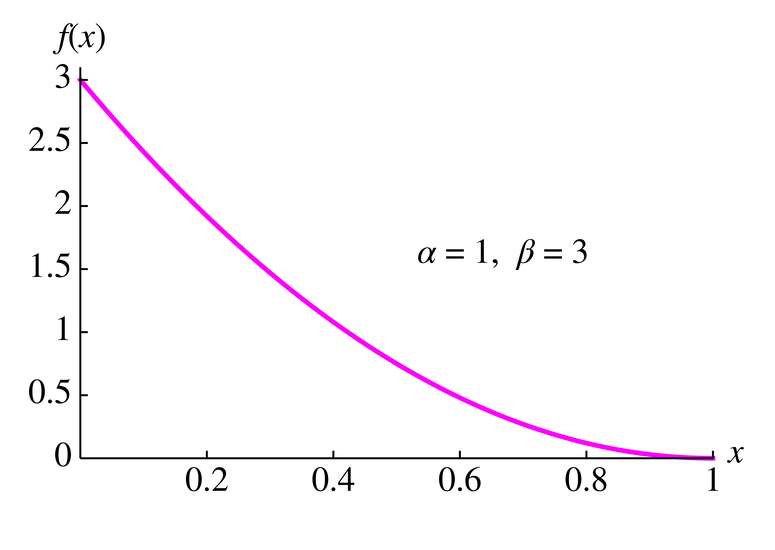
\includegraphics[width=1\linewidth]{beta.png}
Beta. Ofrece modelos satisfactorios para v.a.c.s que toman valores entre dos puntos conocidos.
\begin{equation}\begin{matrix}
f(x)=\begin{cases}\frac{1}{B(\alpha,\beta)}x^{\alpha-1}(1-x)^{\beta-1},\ 0<x<1,\\\text{de otro modo,}\ 0,\end{cases}\\
\text{donde } B(\alpha,\beta)=\\
\int_{0}^{1}x^{\alpha-1}(1-x)^{\beta-1}dx=\\
(\Gamma(\alpha)\Gamma(\beta)\big)/\big(\Gamma(\alpha+\beta)\big)\\
\text{es la función beta.}\\
E(X)=\frac{a}{\lambda},\ Var(X)=\frac{a}{\lambda^2}
\end{matrix}\end{equation}\end{subfigure}
\end{figure}